\documentclass[14pt, aspectratio=169, handout]{beamer}
\usetheme{Copenhagen}
\usecolortheme{seahorse}
\setbeamertemplate{navigation symbols}{}
\setbeamertemplate{headline}{}

%\usepackage{pgfpages}
%\pgfpagesuselayout{4 on 1}[a4paper, border shrink=5mm]

\usepackage{graphicx} % Required for inserting images
\usepackage{multicol}
%\usepackage{enumitem}
\usepackage{amsfonts}
\usepackage{amsmath}
\usepackage{xcolor}
\definecolor{myblue}{RGB}{0, 0, 255} 
\definecolor{mygreen}{RGB}{0, 180, 80}
\definecolor{myred}{RGB}{153, 0, 0}
\definecolor{myorange}{RGB}{255, 153, 51}
\definecolor{mypurple}{RGB}{102, 0, 204}
\usepackage{tikz}

%--- commands for transform arrows----------------
\newcommand{\transform}[2]{%
    \begin{tikzpicture}
        % Open circle
        \draw[thick] (0,0) circle (0.1);
        % Line with number above and adjustable length
        \draw[thick] (0.1,0) -- (#2,0) node[midway, above] {#1};
        % Filled circle
        \filldraw[thick] (#2,0) circle (0.1);
    \end{tikzpicture}%
}
\newcommand{\invtransform}[2]{%
    \begin{tikzpicture}
        % filled circle
        \filldraw[thick] (0,0) circle (0.1);
        % Line with number above and adjustable length
        \draw[thick] (0.1,0) -- (#2 -0.1,0) node[midway, above] {#1};
        % open circle
        \draw[thick] (#2,0) circle (0.1);
    \end{tikzpicture}%
}
\newcommand{\verticaltransform}[4]{%
    \begin{tikzpicture}
        % Open circle at the bottom with text below
        \filldraw[thick] (0,0) circle (0.1) node[below=3pt] {$#4$};
        % Vertical line with number on the left
        \draw[thick] (0,0.1) -- (0,#2 -0.1) node[midway, left] {#1};
        % Filled circle at the top with text above
        \draw[thick] (0,#2) circle (0.1) node[above=3pt] {$#3$};
    \end{tikzpicture}%
}
\newcommand{\verticalinvtransform}[4]{%
    \begin{tikzpicture}
        % Open circle at the bottom with text below
        \draw[thick] (0,0) circle (0.1) node[below=3pt] {$#4$};
        % Vertical line with number on the left
        \draw[thick] (0,0.1) -- (0,#2) node[midway, left] {#1};
        % Filled circle at the top with text above
        \filldraw[thick] (0,#2) circle (0.1) node[above=3pt] {$#3$};
    \end{tikzpicture}%
}

\definecolor{darkblue}{RGB}{0, 0, 139}
\definecolor{lightblue}{RGB}{173, 216, 230}

\title{SST1 Übungsstunde 7}
\author{Matteo Dietz}
\date{November 2024}

\begin{document}

\maketitle

\begin{frame}{Themenüberblick}
    \begin{itemize}
        \item \textbf{Spezielle Eingangssignale von LTI-Systemen}:
        \item[] Repetition: Fourierreihen
        \item[] Plancherel und Parseval für periodische Signale
        \item[] 
        \item \textbf{Anwendungen der FT auf LTI-Systeme}:
        \item[] Ideale Tiefpassfilter
        \item[] Bandbegrenzte Signale
    \end{itemize}
\end{frame}


\begin{frame}{Aufgaben für diese Woche}
    \begin{itemize}
        \item[] \textbf{67}, \textbf{68}, 69, \textbf{70}, 71, \textbf{72}, 73, 74, 75, \textbf{76}, \textbf{77}
        \item[] 
        \item[] 69-74 waren schon letze Woche dabei.
        \item[] 
        \item[] Die \textbf{fettgedruckten} Übungen empfehle ich, weil sie wesentlich zu eurem Verständnis der Theorie beitragen und/oder sehr prüfungsrelevant sind.
    \end{itemize}
\end{frame}

\begin{frame}{Repetition: Fourierreihen}
    \fcolorbox{darkblue}{lightblue}{%
    \parbox{\dimexpr\linewidth-2\fboxsep-2\fboxrule\relax}{
        $$x(t) = x(t + T) = \sum_{k=-\infty}^{\infty} c_k e^{\frac{2 \pi i k t}{T}}, \hspace{12pt} \text{wobei} \hspace{12pt} c_k = \frac{1}{T}\int_0^T x(t) e^{-\frac{2 \pi i k t}{T}} \text{d}t$$
          \hspace{40pt} $x(t)$ wird gemäss Nr. 21 fouriertransformiert zu:
        $$(\mathcal{F}x)(f) = \hat{x}(f) = \mathcal{F}\left\{ \sum_{k = -\infty}^{\infty} c_k e^{\frac{2 \pi i k t}{T}}\right\} = \sum_{k = -\infty}^{\infty} c_k \delta\left( f - \frac{k}{T} \right)$$
    }}%
\end{frame}

\begin{frame}{Fourierreihen: Eigenschaften}
    \begin{itemize}
        \item[(i)] Fourierreihen existieren nur für periodische Signale.
        \item[] 
        \item[(ii)] Periodische Signale haben immer ein "diskretes" Frequenzspektrum.
        \item[] 
        \item[(iii)] $c_k$ sind die komplexen Koeffizienten und beschreiben das Signal im Frequenzbereich.
    \end{itemize}
\end{frame}

\begin{frame}{Periodische Signale an LTI-Systemen}
    \begin{itemize}
        \item Eingangssignal: $x(t) = \displaystyle\sum_{k = -\infty}^{\infty} c_k e^{\frac{2 \pi i k t}{T}}$
        \item[] 
        \item Dank Linearität, Stetigkeit und weil $\left(H \displaystyle e^{2 \pi i f_0 \cdot}\right)(t) = \hat{h}(f_0) e^{2 \pi i f_0 t}$
        \item[]
        \item[] \fcolorbox{darkblue}{lightblue}{%
    \parbox{\dimexpr\linewidth-2\fboxsep-2\fboxrule\relax}{
        $$\hspace{-30pt} \implies y(t) = (Hx)(t) = \sum_{k = -\infty}^{\infty} \smash{\underbrace{c_k \hat{h}\left(\frac{k}{T}\right)}_{d_k}} e^{\frac{2 \pi i k t}{T}}$$
        \vspace*{0.15cm}
    }}%
    \item[] 
    \item Das Ausgangssignal auf ein $T-$periodisches Eingangssignal ist auch $T-$periodisch.
    \end{itemize}
\end{frame}

\begin{frame}{Poissonsche Summenformel}
\fcolorbox{darkblue}{lightblue}{%
    \parbox{\dimexpr\linewidth-2\fboxsep-2\fboxrule\relax}{
        $$\hspace{12pt} \sum_{k=-\infty}^\infty h(t-kT) = \frac{1}{T} \sum_{k=-\infty}^\infty \hat{h}\left(\frac{k}{T}\right)e^{\frac{2\pi i k t}{T}}
        $$
    }}%
    \begin{itemize}
        \item[] 
        \item \textbf{Beispiel}:
        \item[] 
        \item[] 
        \item[] 
        \item[] 
        \item[] 
    \end{itemize}
\end{frame}

\begin{frame}{Plancherel und Parseval für $T-$periodische Signale}
    Es seien $x,y \in L^2([0,T])$ $T-$periodisch. Dann gilt:
    \vspace*{0.25cm}
    \fcolorbox{darkblue}{lightblue}{%
    \parbox{\dimexpr\linewidth-2\fboxsep-2\fboxrule\relax}{
    \begin{center}
        \textbf{Plancherelsche Identität für periodische Signale} 
    \end{center}
    $$\frac{1}{T}\int_0^T x(t)y^\ast(t) \text{d}t = \sum_{k=-\infty}^\infty c_k^x \left( c_k^y \right)^\ast$$
    \begin{center}
        \textbf{Parsevalsche Beziehung für periodische Signale}
    \end{center}
    $$||x||^2_{L^2([0,T])} = \frac{1}{T} \int_0^T |x(t)|^2 \text{d}t = \sum_{k=-\infty}^\infty |c_k|^2$$
    }}
\end{frame}

\begin{frame}{Parseval: Bemerkungen}
    \begin{itemize}
        \item Wir betrachten hier den Fall $T=1$. 
        \item[] 
        \item Die Parsevalsche Beziehung sagt zwei Dinge aus: \begin{enumerate}
            \item[] 
            \item Die $L^2$-Norm der Funktion (“Energie”) kann statt aus einem Integral aus einer Summe (der Fourier-Koeffizienten im Betragsquadrat) berechnet werden.
            \item[] 
            \item Die Fourierkoeffizenten klingen für $L^2([0,1])$ schneller als $\frac{1}{n}$ ab.
        \end{enumerate} 
    \end{itemize}
\end{frame}

\begin{frame}{Parseval: Bemerkungen}
    \begin{itemize}
        \item Wir leiten $x(t) = \displaystyle\sum_{k = -\infty}^\infty c_k e^{2 \pi i k t}$ nach $t$ ab:
        $$\frac{\text{d}x(t)}{\text{d}t} = \sum_{k=-\infty}^{\infty} 2 \pi i k \underbrace{\cdot c_k \cdot}_{\hat{x}(k)} e^{2 \pi i k t}$$
        $ \implies$ für die Fourier-Koeffizienten der Ableitung von $x(t)$ gilt: $\hat{x'}(k) = 2 \pi i k \hat{x}(k)$ und somit:
        $$\widehat{x^{(n)}}(k) = (2 \pi i k)^n \underbrace{\hat{x}(k)}_{c_k} \hspace{12pt} \text{und} \hspace{12pt} ||x^{(n)}||^2_{L^2} = (2 \pi)^{2n} \sum_{k = -\infty}^\infty k^{2n}|\underbrace{\hat{x}(k)}_{c_k}|^2,$$
    \end{itemize}
\end{frame}

\begin{frame}{Parseval: Bemerkungen}
    \begin{itemize}
        \item Direkte Verbindung zwischen Glattheit eines Signals und dem Abfall seiner Fourier-Koeffizienten:
        \item[]
        \item Je glatter das Signal, desto schneller ist der Abfall seiner Fourier-Koeffizienten, also desto schneller ist die Konvergenz der Fourierreihe.
        \item[]
        \item \textbf{Anwendung}: Sehr gute numerische Approximation von glatten Funktionen mittels kurzen Fourier-Summen. Unglatte Funktionen brauchen längere Fourier-Summen.
    \end{itemize}
\end{frame}

\begin{frame}{Aufgaben}
    \begin{itemize}
        \item \textbf{Prüfungsaufgabe: Frühjahr 2024, Aufgabe 1.a) iii, iv und 1.d)i, ii}
    \end{itemize}
\end{frame}

\begin{frame}{Anwendung der FT auf LTI-Systeme}
\vspace*{-0.5cm}
   \begin{center}
    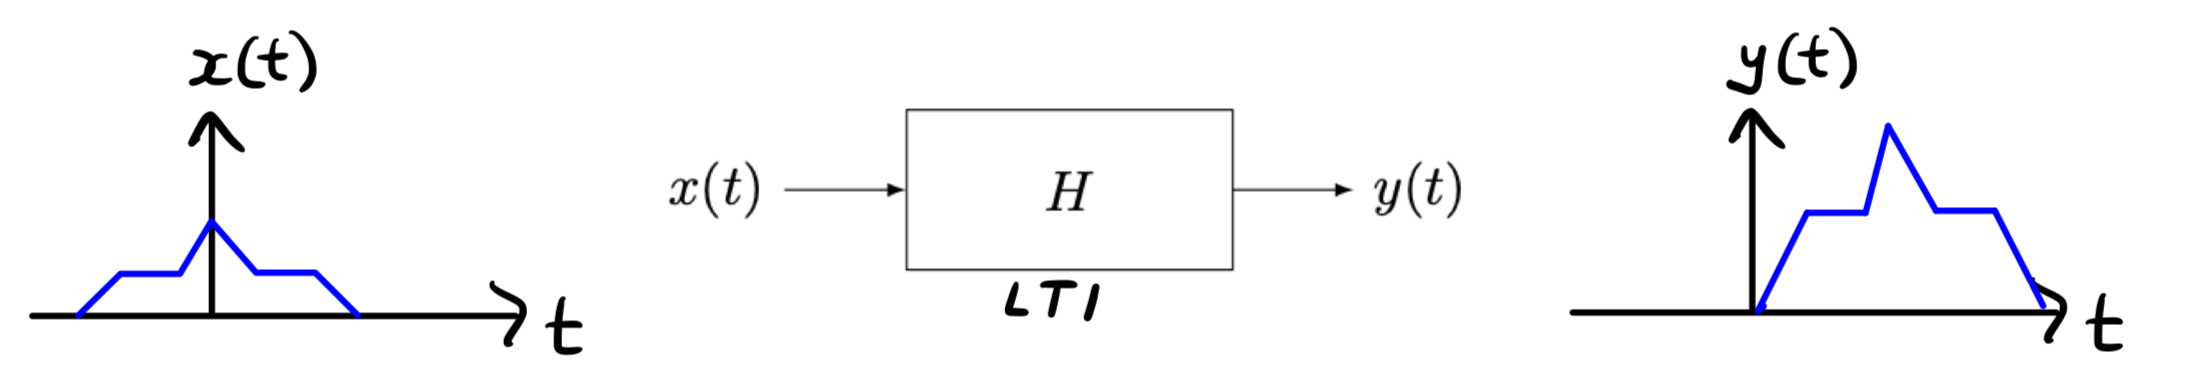
\includegraphics[width=0.7\linewidth]{figures/Verzerrungsfrei.jpg}
\end{center}
\vspace*{-0.5cm}
\textbf{Def}: Ein \textbf{verzerrungsfreies} System hat folgende Eigenschaften:
\vspace*{0.25cm}
\begin{enumerate}
    \item Input und Output haben die gleiche Form, d.h.\\
    $y(t) = kx(t-t_0) \; \transform{2.}{1.5} \; \hat{y}(f) = \underbrace{ke^{-2\pi i f t_0}}_{= \hat{h}(f)}\hat{x}(f)$
    \item $\hat{h}(f) = |\hat{h}(f)|e^{i \varphi(f)} = k e^{i(-2 \pi f t_0)} \; \invtransform{}{1.5} \; h(t) = k \delta(t-t_0)$
    \item Das System ist linear, stabil, kausal und zeitinvariant
\end{enumerate}
\end{frame}

\begin{frame}{Tiefpassfilter: Beispiel}
    \vspace*{-0.25cm}
    \begin{center}
        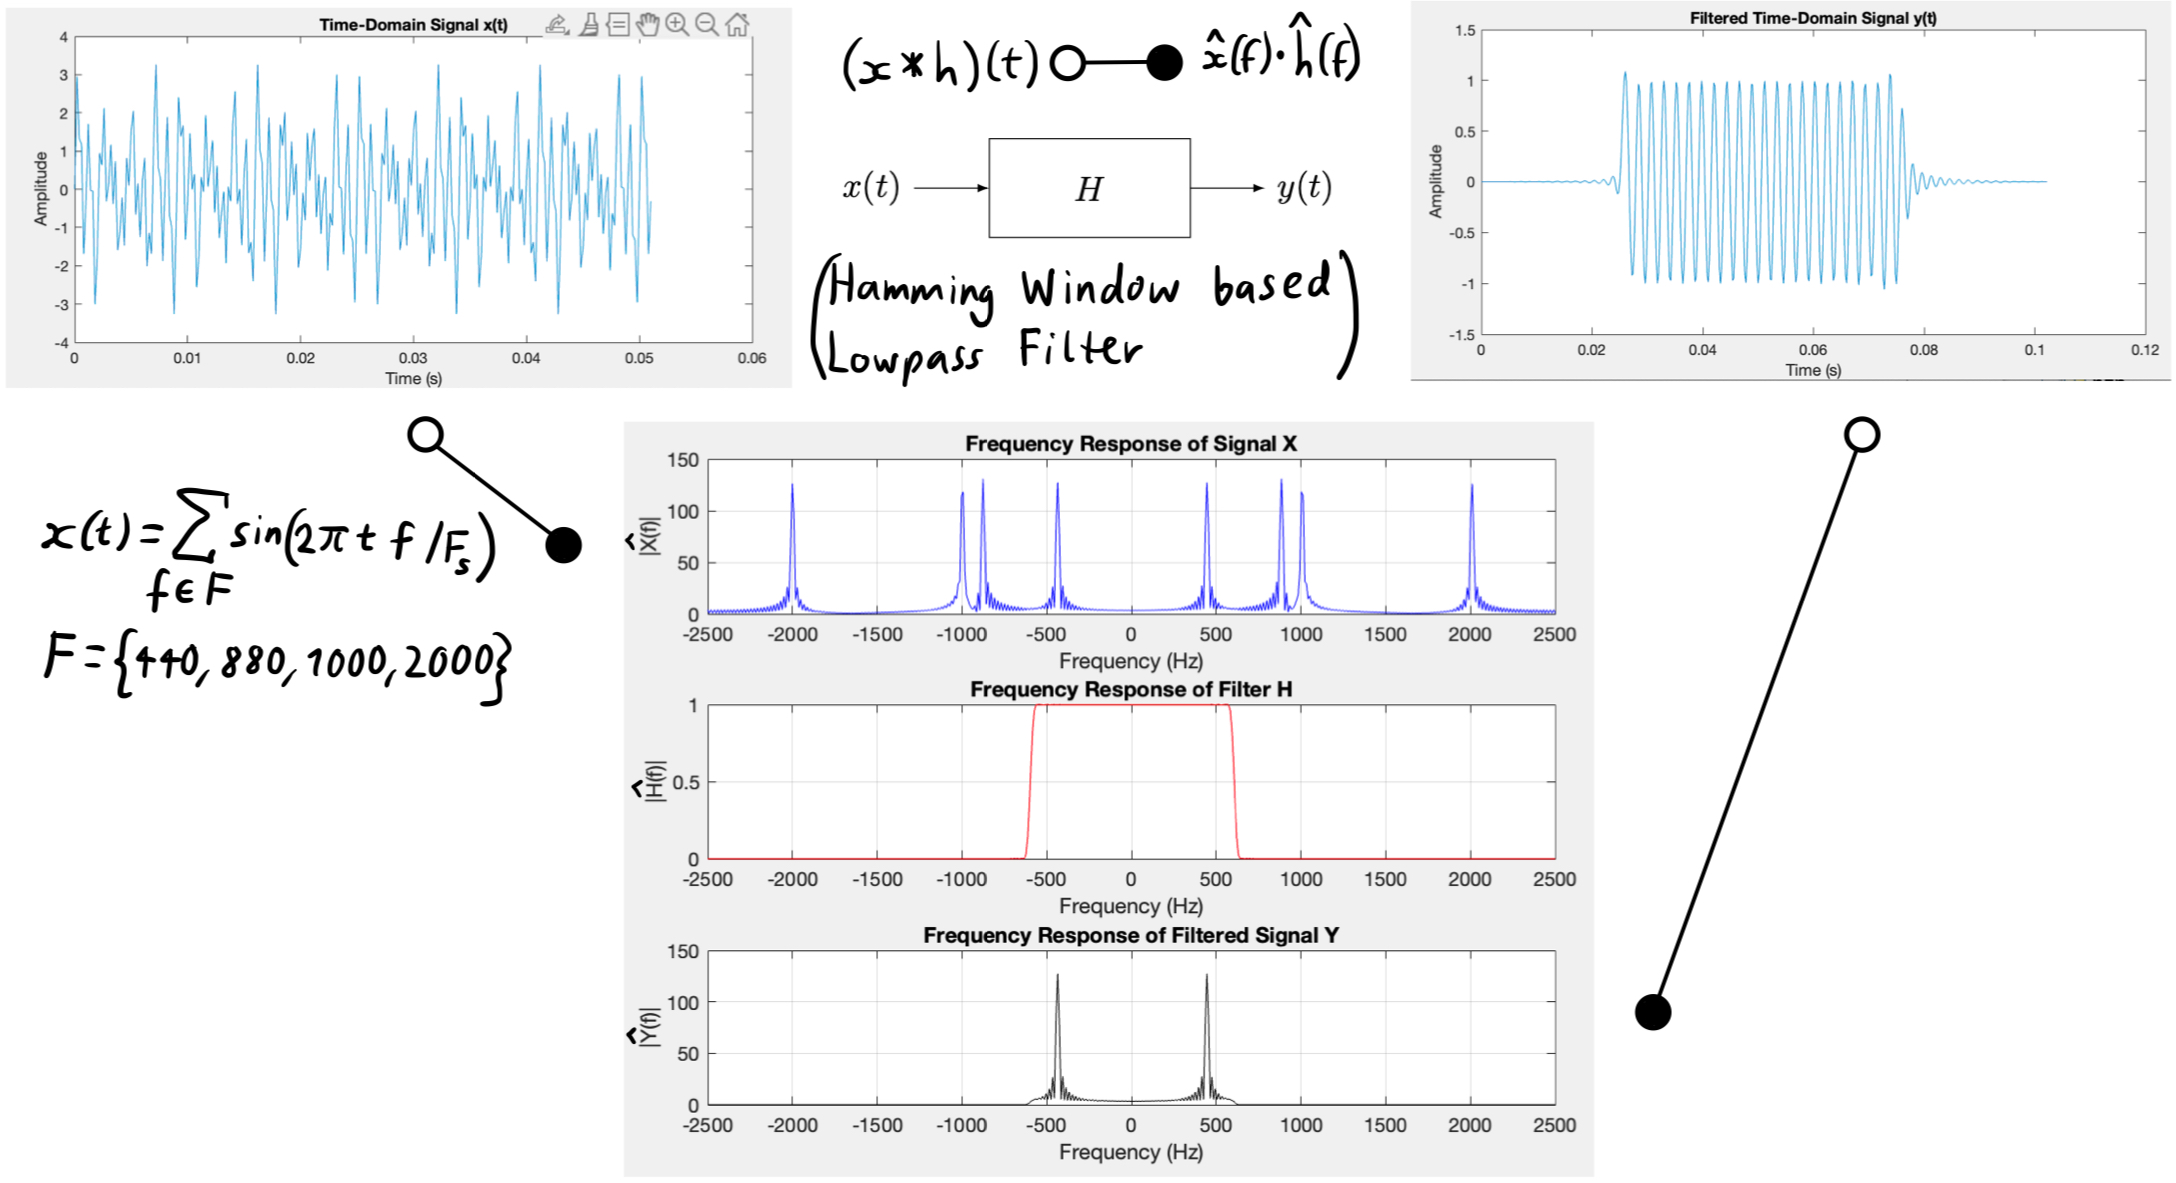
\includegraphics[width=0.98\linewidth]{figures/Hamming_lp.jpg}
    \end{center}
\end{frame}

\begin{frame}{Idealisierte Tiefpassfilter}
\begin{center}
    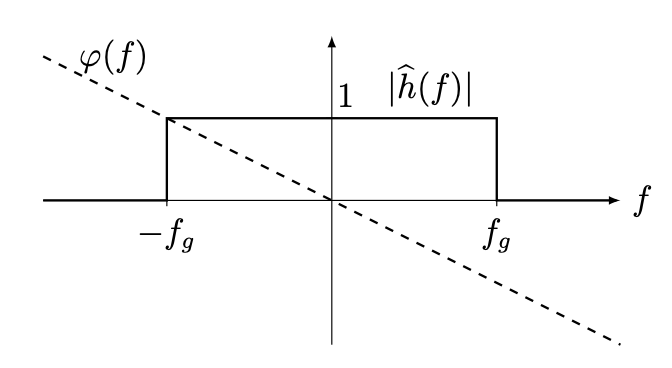
\includegraphics[width=0.6\linewidth]{figures/h_id_freq.png}
\end{center}
    $$\hat{h}(f) = |\hat{h}(f)|e^{i \varphi(f)}, \hspace{10pt} \text{wobei} \hspace{10pt} |\hat{h}(f)|= \begin{cases}
    1, \; |f| \leq f_g\\
    0, \; \text{sonst}
    \end{cases} \hspace{12pt} \varphi(f) = -2 \pi f t_0$$
\end{frame}

\begin{frame}{Idealisierte Tiefpassfilter}
    \begin{itemize}
    \item $e^{i\varphi(f)}$ entspricht einer Zeitverzögerung von $t_0$.
    \item[] 
    \item Wir schreiben $h(t) = \underbrace{|\hat{h}(f)|}_{=:\hat{h}_{id}(f)} e^{-2\pi i f t_0} \; \invtransform{2.}{1.5} \; h_{id}(t-t_0)$
    \item[] 
    \item $h_{id}(t) = \displaystyle\frac{\sin(2 \pi f_g t)}{\pi t} \; \transform{27.}{1.5} \; \hat{h}_{id}(f) = \displaystyle\begin{cases}
        1, |f| \leq f_g\\
        0, \; \text{sonst}
    \end{cases}$ 
    \item[] 
    \item $ \implies h(t) = h_{id}(t-t_0) = \displaystyle\frac{\sin(2 \pi f_g (t-t_0))}{\pi (t-t_0)}$
\end{itemize}
\end{frame}

\begin{frame}{Idealisierte Tiefpassfilter: Bemerkungen}
    \begin{enumerate}
    \item Da $h(t) = 0 \; \forall t < 0$ \textbf{nicht gilt}, ist das ideale Tiefpassfilter \textcolor{red}{\textbf{nicht kausal}}.
    \item[] 
    \item Es gilt \textbf{nicht}, dass $\displaystyle\int_{-\infty}^{\infty} |h(t)|\text{d}t < \infty$. \\$\implies$ ideales Tiefpassfilter ist \textcolor{red}{\textbf{nicht BIBO-stabil}}.
    \item[] Grund: Riemann-Lebesgue Lemma
    \item[] 
    \item[1.\&2.] $\implies$ Ideale Tiefpassfilter sind \textcolor{red}{\textbf{nicht realisierbar}} in der Praxis. Wir müssen das Filter kausal und BIBO-stabil machen!
\end{enumerate}
\end{frame}

\begin{frame}{Tiefpassfilter: Kausalisierung}
    \begin{itemize}
    \item Wir wollen Kausalität: $h(t) = 0 \; \forall t < 0$
    \item[] 
    \item Im Zeitbereich: $h_{id}(t) = \displaystyle\frac{\sin(2 \pi f_g t)}{\pi t}$
    \item[] 
    \item Wir verschieben $h_{id}(t)$ um $t_1$,  multiplizieren mit $\sigma(t)$ und erhalten $h(t) = 0 \; \forall t < 0$.
    \item[] 
    \item Somit $h_{kaus}(t) = h_{id}(t-t_1)\sigma(t)$
    \end{itemize}
\end{frame}

\begin{frame}{Tiefpassfilter: Kausalisierung}
    \begin{center}
        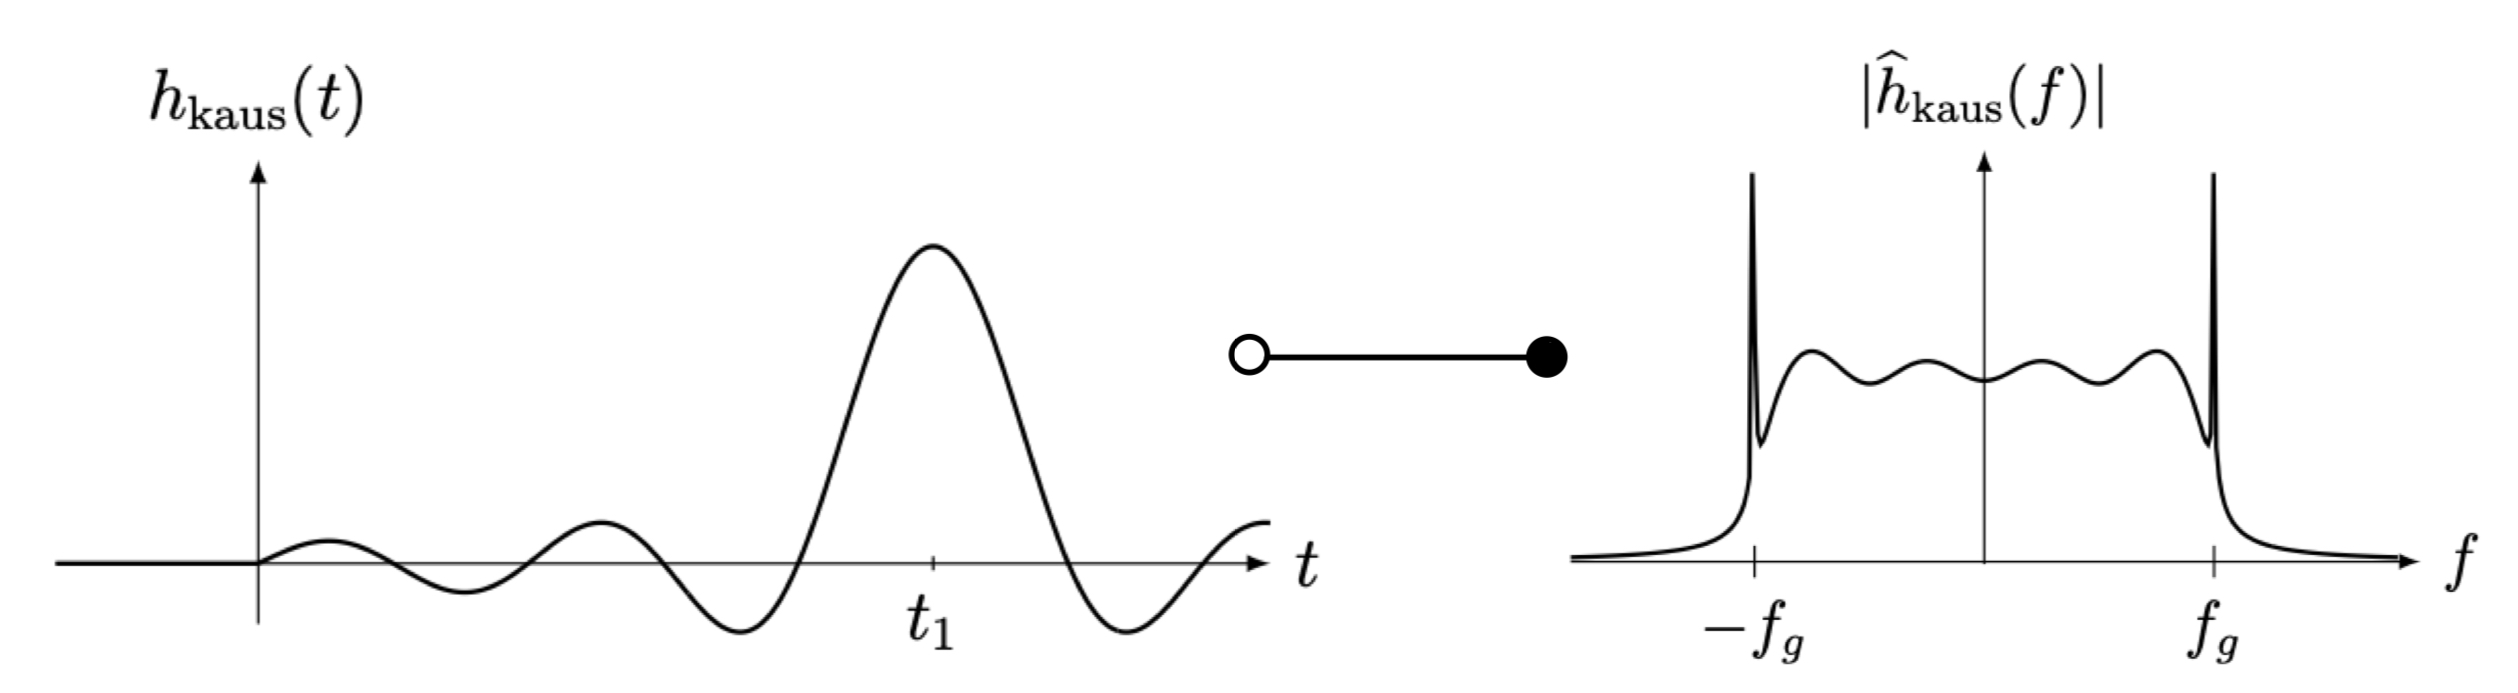
\includegraphics[width=0.8\linewidth]{figures/h_kausal.jpg}
    \end{center}
    \begin{itemize}
    \item Die dazugehörige Fouriertransformation $\hat{h}_{kaus}(f)$ verstärkt die Frequenzen bei $\pm f_g$ deutlich. 
    \item[] 
    \item $\implies h_{kaus}$ ist kein gutes Filter.
    \end{itemize}
\end{frame}

\begin{frame}{Tiefpassfilter: Stabilisierung}
    \begin{itemize}
    \item Wir wollen $h(t)$ absolut integrierbar. Wir falten $(\hat{h}_{id}\ast \hat{h}_{ge}) (f)$
    \item[] \begin{center}
        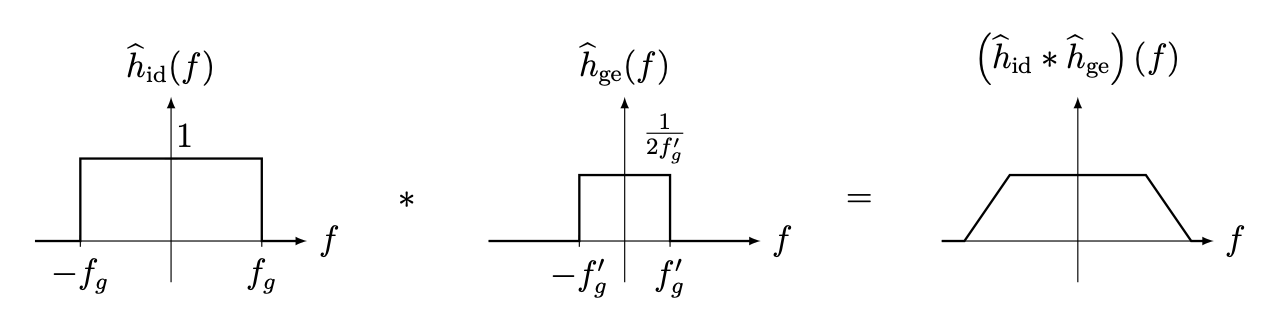
\includegraphics[width=0.9\linewidth]{figures/h_stabil_freq.png}
    \end{center}
    \item Wir erhalten: $$(\hat{h}_{id} \ast \hat{h}_{ge})(f) \; \invtransform{}{1.5} \; h_{id}(t) h_{ge}(t) \propto \displaystyle\frac{1}{t} \cdot \displaystyle\frac{1}{t} = \displaystyle\frac{1}{t^2} \in L^1$$
    \end{itemize}
\end{frame}

\begin{frame}{Tiefpassfilter: Stabilisierung}
    \begin{itemize}
        \item Das resultierende Tiefpassfilter ist BIBO-stabil und sieht im Frequenzbereich aus wie folgt:
        \item[] \begin{center}
        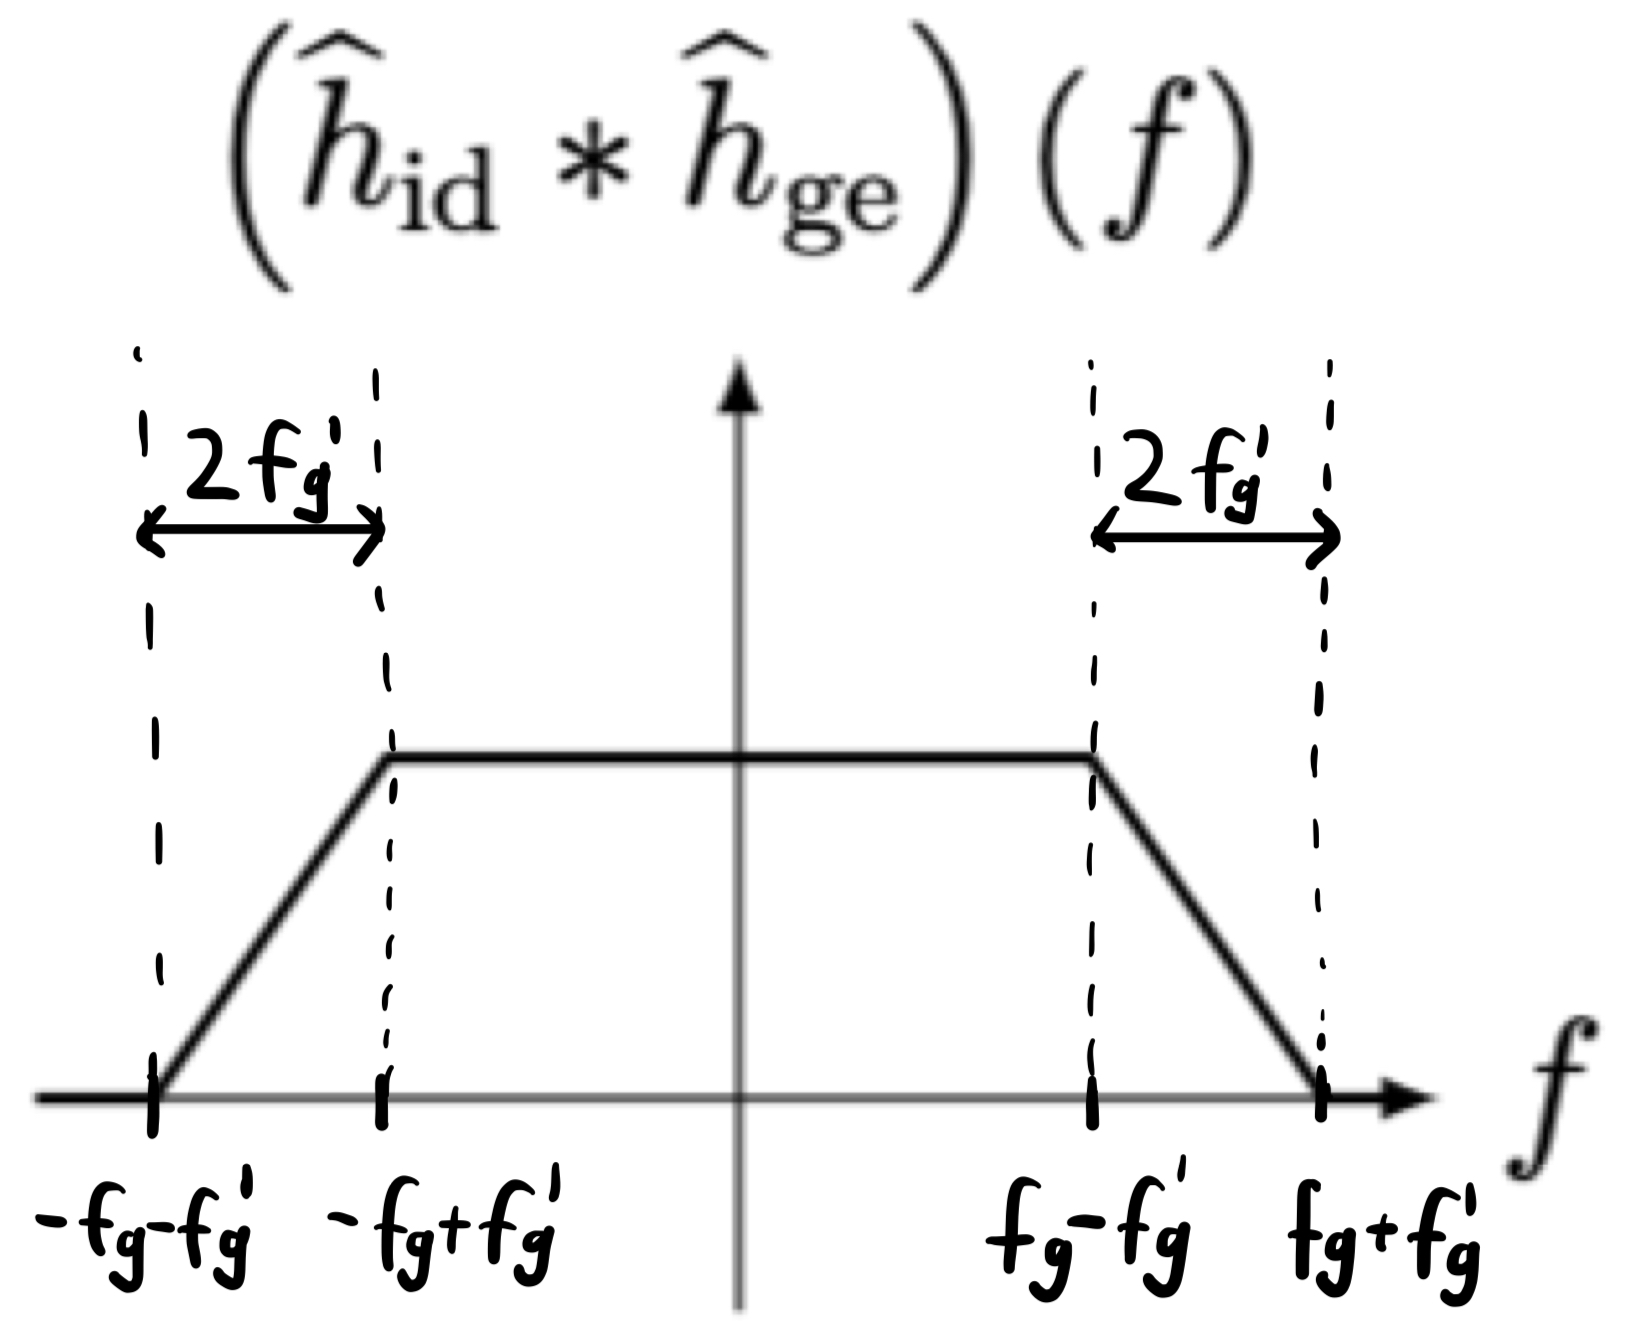
\includegraphics[width=0.3\linewidth]{figures/h_stabil_2.jpg}
        \end{center}
        \item Da dieses Filter nicht perfekt ist in den Bereichen $|f \pm f_g| \in [-f_g', f_g']$, versucht man $f_g'$ so klein wie möglich zu wählen.
    \end{itemize}
\end{frame}

\begin{frame}{Bandbegrenzte Signale}
    \begin{itemize}
    \item \textbf{Def}: Die \textbf{Bandbreite} des Signals $x$ ist das kleinste $W$, so dass
    $$(x \ast h_{\text{TP,}W})(t) = x(t), \hspace{12pt} \text{für alle } t \in \mathbb{R}, \text{ wobei}$$
    $$h_{\text{TP,}W}(t) = \sin (2 \pi W t)/(\pi t).$$
    \item Im Frequenzbereich bedeutet das
    $$\hat{x}(f)\hat{h}_{\text{TP,}W}(f) = \hat{x}(f), \hspace{12pt} \text{für alle }f\in \mathbb{R}, \text{ und}$$
    $$\hat{h}_{\text{TP,}W}(f) = \begin{cases}
        1, \; |f| \leq W \\
        0, \; \text{sonst.}
    \end{cases}$$
    \end{itemize}
\end{frame}

\begin{frame}{Bandbreite}
    \begin{itemize}
        \item \textbf{Intuitiv}: Die Bandbreite ist die betragsweise höchste Frequenz (positiv oder negativ), die in einem Signal enthalten ist.
        \item[] 
        \item[] \begin{center}
            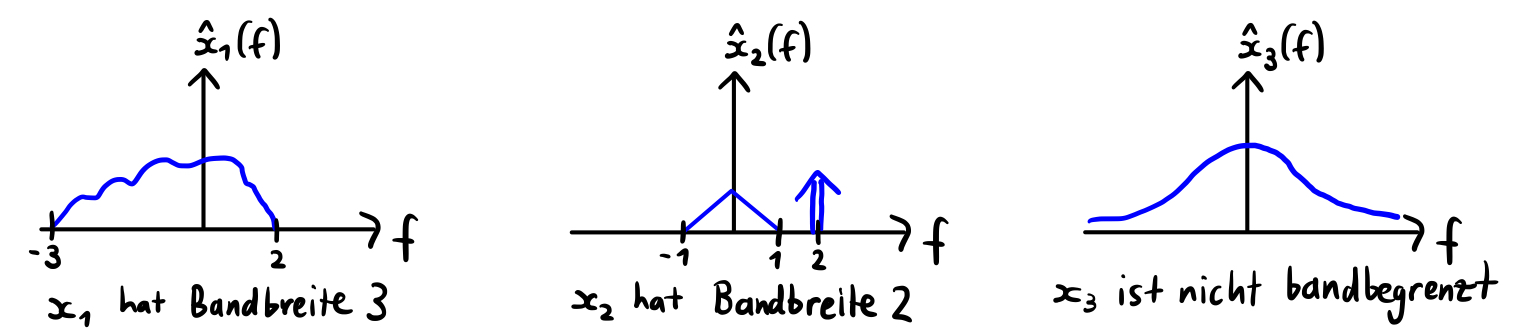
\includegraphics[width=\linewidth]{figures/Bandbreite.jpg}
        \end{center}
    \end{itemize}
\end{frame}

\begin{frame}{Bandbreite: Bemerkungen}
    \begin{itemize}
        \item Seien $x_1, x_2$ zwei Signale mit Bandbreite $W_1$ resp. $W_2$ \begin{itemize}
        \item[] 
        \item[(i)] $x_1(t) + x_2(t)$ hat Bandbreite max$\{W_1, W_2\}$
        \item[] 
        \item[(ii)] $(x_1 \ast x_2)(t)$ hat Bandbreite min$\{W_1, W_2\}$
        \item[] 
        \item[(iii)] $x_1(t)x_2(t)$ hat Bandbreite $\leq W_1 + W_2$
    \end{itemize}
    \end{itemize}
\end{frame}

\begin{frame}{Bernstein'sche Ungleichung}
    \textbf{Thm}: Wenn $x(t)$ in der folgenden Form dargestellt werden kann: $$x(t) = \displaystyle\int_{-W}^W g(f)e^{2 \pi i f t} \text{d}f, \text{ für alle } t\in \mathbb{R}$$ wobei $g$ eine absolut integrierbare Funktion ist, d.h. $g\in L^1$, dann:  $$\left| \frac{\text{d}x(t)}{\text{d}t} \right| \leq 4 \pi W \sup_{\tau \in \mathbb{R}}|x(t)|, \hspace{12pt} \text{für alle } t \in \mathbb{R}.$$
\end{frame}

\begin{frame}{Bernstein'sche Ungleichung}
    \begin{itemize}
    \item Dieses Kriterium liefert uns eine Abschätzung für die Ableitung von $x(t)$.
    \item[] 
    \item Kleine Bandbreite $W \implies$ nur tiefe Frequenzen sind im Signal enthalten $\implies x(t)$ kann sich nur "langsam" ändern.
\end{itemize}
\end{frame}

\begin{frame}{Aufgabe 68}
    
\end{frame}

\end{document}
